\chapter{Introduction}
\section{Context}
\subsection{Overview of Climate Modeling and Seasonal Forecasting}\begin{titlepage}
    \centering



%
%\fbox{\begin{minipage}{0.9\textwidth}
%        \centering
%        \Huge
%        \textbf{Evaluation of Climate Models For Seasonal Forecasting in the MENA Region}
%    \end{minipage}} \\



    \Huge
   \textbf{Probabilistic Evaluation of Climate Models For Seasonal Forecasting in the MENA Region} \\

    % Subtitle
    \vspace{0.5cm}
    \Large
    \textbf{Identification of Windows of Opportunity}

    \vspace{0.5cm}
    
    \begin{figure}[H]
    \centering
    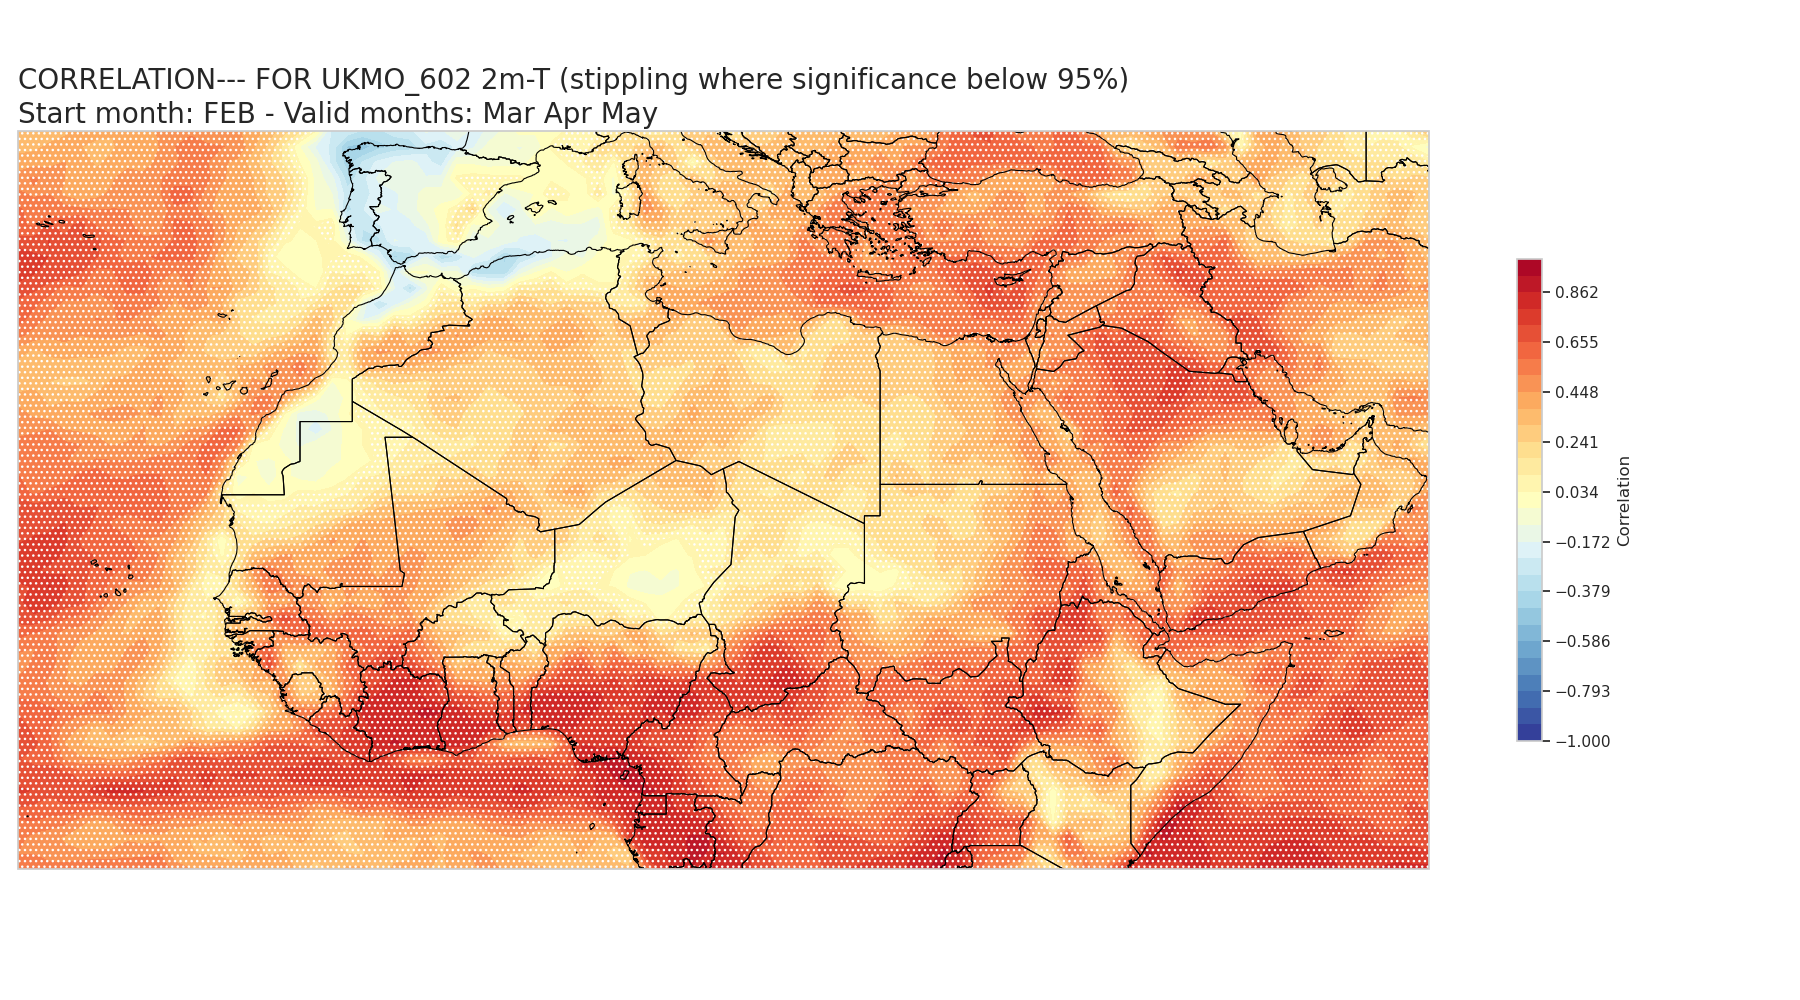
\includegraphics[scale=0.3]{titlepage.png} 
    \end{figure}

    % Author and Supervisors
    \Large
    \textbf{Authors:} \\
    Nohayla BERRAHMOUCH, Mohamed EL-BADRI \\
    \textit{Hassania School of Public Works}

    \vspace{0.5cm}
    \textbf{Supervised by:} \\
    Wafae BADII (Direction Generale de la Meteorologie, Morocco)\\ Nicholas Savage (Met Office, Exeter, UK) \\ Idriss BARI (Direction Generale de la Meteorologie, Morocco)

    \Large
    \textbf{Hassania School of Public Works}

    \vspace{0.8cm}

    % Date (optional)
    \Large
    \textbf{2024}

    \vspace{0.31cm}

    
\end{titlepage}
